\chapter{Implementierung einer energieeffizienten Registerallokation}
\label{chap:Implementierung}
Nachdem die nötigen Grundlagen erläutert sind, soll in diesem Kapitel aufgezeigt werden, wie der Compiler aufgebaut ist und wie das gesetzte Ziel implementiert wurde. Hierzu wird kurz auf den Ausgangsstatus des Codes und dessen Bestandteile eingegangen, um das komplette System besser verstehen zu können. Anschließend wird veranschaulicht, wie mit Hilfe einer optimierten Registerallokation die Verlustleistung gesenkt werden kann und wie dies mit einer Heuristik implementiert wurde. Im Anschluss wird ein genetischer Opimierungsalgorithmus entworfen, implementiert und evaluiert.
\newpage
\section{Instruktion-Scheduler}
 Das folgende Schaubild (siehe Abbildung \ref{fig:flow_compiler}) zeigt den Aufbau, Bestandteile, Ein- und Ausgaben des Schedulers.Die nachfolgenden Bestandteile yu denen auch die in dieser Arbeit relevante Register-Allokation gehoert, sind im Einzelnen detailliert beschrieben.
 Gestartet wird mit einem Assembler-Programm, dass in einer ASM-Datei vorliegt und dem Code übergeben wird.
 
 
%	\begin{wrapfigure}{r}{0.5\textwidth}
%		\begin{center}
%			\includesvg[width=0.48\textwidth]{flowchart}
%		\end{center}
%		\caption{Compiler Ablaufdiagramm}
%		\label{fig:flow_compiler}
%	\end{wrapfigure}


	\begin{figure}[H] 
		\centering
		\includesvg[width=0.5\textwidth]{flowchart}
		\caption{Compiler Ablaufdiagramm}
		\label{fig:flow_compiler}
	\end{figure}

\begin{itemize}
	\item Precompiler\\
		Da der Assembler-Code, Kommentare oder Bestandteile aufweisen kann, die nicht in der eigentlichen Assemblersprache enthalten sind, ist es nötig diese aufzulösen. Dies übernimmt der Precompiler oder Preprozessor der die Konstrukte in einen vom Prozessor ausführbaren Code bzw. Anweisungen umwandelt. Ein Beispiel für ein solches Konstrukt ist das An- und Ausschalten des Schedulings für bestimmte Bereiche des Codes. Hierbei kann dem Compiler, im Assembler-Programm durch Angabe des \"scheduling-off\"-Befehls mitgeteilt werden, welche SLMs vom Scheduling unberührt bleiben sollen.
	\item Virtual Renaming\\
		Im Teil des virtuellen Renaming (Umbenennen) werden die im Assembler-Code vorhandenen virtuellen Register umbenannt, um eine konsistente Allokation und bessere Nachvollziehbarkeit zu gewährleisteten. Außerdem wird in diesem Teil des Compilers überprüft, ob ein virtuelles Register verwendet wurde, bevor dieses zugewiesen wurde. Diese Szenario ist nicht zulässig und muss im Assembler-Programm aufgelöst werden.
	\item Register-Initalisierung\\
		Die Register-Initalisierung iteriert über alle Operationen, dabei werden die Adressen des Register-Files blockiert, welche bereits von physikalischen Registern verwendet werden. Dadurch wird verhindert, dass diese Positionen im weiteren Verlauf für das virtuelle Register-Mapping verwendet werden können.
	\item Scheduling\\
		Wie in den Grundlagen \ref{sec:scheduling} beschrieben, ist das Scheduling zuständig für die Anordnung der Operationen im OP-Code des Prozessor. Dabei wird je nach gewähltem Optimierungsgrad ein anderer Scheduling-Algorithmus gewählt. Hierbei kann zwischen einem genetischen Instruktions-Scheduling und einem Heuristischem-Ansatz entschieden werden. Beide Algorithmen rufen intern die Register-Allokation auf. Wird der genetische Algorithmus verwendet, wird der Fitness-Wert der Register-Zuweisung mit der Bewertungsfunktion des Instruktion-Schedulings verrechnet.
	\item Register Allokation\\
		Die Register-Allokation ist dafür zuständig, dass alle Register, sowohl physikalische als auch virtuelle, im Register-File abgespeichert werden können. Dazu wird diese nach jedem Scheduling einer SLM aufgerufen und durchläuft alle Instruktionen, sowie die darin verwendeten Register. Bei der Verwendung eines physikalischen Registers überprüft die Allokation ob die vom Programmierer gewählte Register-Adresse und Register-File bereits blockiert, oder nicht zuweisbar ist. Handelt es sich um ein virtuelles Register, wird zuerst eine geeignete Adresse zugewiesen. Hierbei wird ebenfalls darauf geachtet, dass diese nicht blockiert oder nicht möglich ist.
		Es existieren auch hier zwei Algorithmen zur Register-Allokation. Zum Einen eine Heuristik (siehe Kapitel \ref{sec:Heuristik}) und zum Andern ein Genetischer Algorithmus (siehe Kapitel \ref{sec:genetischerAlgorithmus}). Beide Algorithmen werden im Folgenden nun näher beleuchtet.
\end{itemize}


\section{Optimierungsansatz durch Register-Allokation}
\label{chap:ansatz}
Das Ziel des Algorithmus ist es, eine geeignete Register-Allokation zu finden, bei der die Verlustleistung minimal wird. Um dies zu erreichen, soll der Freiheitsgrad durch den Einsatz von virtuellen Registern ausgenutzt werden.
Damit die Verlustleistung des Prozessors gesenkt werden kann, ist es nötig einen Zusammenhang zwischen der Register-Allokation und der Leistungsaufnahme zu finden. Da die Verlustleistung nicht direkt zur Compilezeit bestimmt werden kann, ist eine Metrik nötig die mit dieser korreliert.
Nach genauerem Betrachten der Formel für die dynamische Verlustleistung (siehe Formel \ref{eq:dynVerlustleistung}), hängt diese von vier Faktoren ab: Schaltaktivitäten,  Lastkapazität, Versorgungsspannung und der Frequenz. Da der KUVAKA-Prozessor aus Hardwaresicht bereits fertig entwickelt und optimiert wurde, wird die statische Verlustleistung nicht weiter betrachtet, da diese  nur durch eine Veränderung der Hardware verändert werden kann. Da ebenfalls  die Spannung und Frequenz von der Architektur abhängt, können auch diese  hardware-relevanten Faktoren durch eine Software-Anpassung nicht weiter optimiert werden. Im Folgenden wird nun erst darauf eingegangen, wie durch Minimierung der Schaltaktivitäten die Verlustleistung optimiert werden kann. Im weiteren Verlauf des Textes wird dann ebenfalls der Einfluss der Lastkapazitäten überprüft.\\
Um in ein Register zu schreiben, muss eine geeignete Adresse an den Adressbus angelegt werden. Da es sich bei der Architektur um 2x32 Register handelt, muss für jedes Register eine 5-bit Adresse angelegt werden.
Da der Prozessor zusätzlich über zwei Issue-Slots verfügt, müssen pro Slot ein Target- und zwei Source-Register adressiert werden. Hierbei können die Instruktionen auf Register-File 0 oder 1 schreiben bzw. lesen. Aus diesem Grund besitzt jedes der Register-Files vier Lese- und zwei Schreibports. Die Zuordnung der Issues auf die Register können aus den Tabellen \ref{fig::schreib-port}+\ref{lese-port} entnommen werden.
Schreibt nun beispielsweise eine Instruktion an die Adresse Null und die nachfolgende Instruktion an die Adresse 31 des selben Ports, so wäre dies der Worst-Case, da in diesem Fall alle 5-Bit umgeladen werden müssten. Im Best-Case wurde nur eine Adress-Leitung toggeln.\\
Durch den Einsatz von virtuellen Register (Kapitel \ref{sub:virtuelleR}) können Instruktionen an beliebigen Adressen und Register-Files schreiben bzw. lesen. Durch diese Änderung ist es möglich, die Schaltaktivitäten des Adressbus zu verringern und die Register an eine Position zu alokieren, welche für die Schaltaktivität optimal ist.\\
In der bestehenden Implementierung wurde diese Zuweisung der Register so geregelt, dass die Register-Files immer von einer Seite befüllt wurden. Die Auswahl des Register-Files wurde hierbei über die Anzahl der freien Register-Adressen ermittelt und dasjenige File mit der höheren Anzahl an freien Adressen verwendet. Außerdem wurde bei der Zuweisung darauf geachtet, dass es weiterhin möglich ist X2-Befehle und MAC-Operationen zu bedienen.\\
Um nun dieses Mapping auf die Schaltaktivität und somit auch auf die Verlustleistung zu optimieren, wurde eine neue Heuristik implementiert.
Diese optimiert die Anzahl der Schaltaktivität anhand der Hamming-Distanz.
Die Hamming-Distanz ist nach dem amerikanischen Mathematiker Richard Wesley Hamming benannt und gibt ein Maß für die Unterschiedlichkeit zweier Zeichenketten an. Hierbei ist die Hamming-Distanz die Anzahl der unterschiedlichen Stellen beider Codewörter.
\begin{equation}
00100 \text{ und } 00001 \rightarrow \text{Hamming-Distanze}= 2
\label{eq:hammingdistanze}
\end{equation}
 
\section{Heuristik}
\label{sec:Heuristik}
Um die Hamming-Distanz berechnen zu können, werden die Adressen der letzten adressierten Register gespeichert. Da die Architektur, wie bereits erwähnt, zwei Issue-Slots aufweist und diese auf beide Register-Files zugreifen können, müssen dementsprechend vier Target- und acht Source-Adressen abgespeichert werden (siehe Abbildung \ref{fig:reg_orga}).\\
Hierbei werden nur die Adressen innerhalb einer SLM optimiert, da das Scheduling der einzelnen SLMs parallel in mehrere Threads aufgeteilt ist. Dadurch wuerden Datenabhaenigkeiten bei der Register-Allokation entstehen. Da jedoch SLMs meist sehr groß ausfallen, fallen die nicht optimalen Adress-Toggel nicht stark ins Gewicht. 
Durch den Einsatz einer Architektur mit Adresse-Isolation (siehe Kapitel \ref{subsec:add_iso}), bleiben die zuvor verwendeten Adressen an den Register-File Ports angelegt. Um die Schaltaktivität zu minimieren, wird nun bei jedem virtuellen und physikalischen Register die Hamming-Distanz zu der zuletzt angelegten Adresse des jeweiligen Ports berechnet. Hierbei wird die Adresse auf das Register gemappt, welches die geringste Hamming-Distanz zur zuletzt verwendeten Adresse des selbingen Ports aufweist.\\

\begin{algorithm}[H]
	\begin{algorithmic}[1]
		\STATE {:0 \textbf {ADD} V0R0 V0R0 V0R0 \hspace{50pt}:1 \textbf {OR} V1R0 V0R0 V0R0}
		\STATE {:0 \textbf {ADD} V0R2 V0R0 V0R0 \hspace{50pt}:1 \textbf {OR} V1R2 V0R0 V0R0}
		\STATE {:0 \textbf {ADD} V0R4 V0R0 V0R0 \hspace{50pt}:1 \textbf {OR} V1R4 V0R0 V0R0}
		\STATE {:0 \textbf {ADD} VxR0 V0R0 V0R0 \hspace{50pt}:1 \textbf {OR} VxR1 V0R0 V0R0}
		\STATE {:0 \textbf {ADD} VxR2 VxR0 VxR1 \hspace{50pt}:1 \textbf {OR} VxR0 VxR0 VxR1}
		\caption{Heuristik Beispiel}
		\label{code:heuristik}
\end{algorithmic}
\end{algorithm}

\begin{figure}[H] 
	\centering
	\includesvg[width=\textwidth]{heuristik}
	\caption{Heuristik Beispiel}
	\label{fig:heuristik}
\end{figure}

Anhand des Codebeispiels \ref{code:heuristik} und der Abbildung \ref{fig:heuristik} mit den bereits allokierten Register soll nun das Mapping der virtuellen Register verdeutlicht werden.
Der Code zeigt hierbei einen bereist geschedulten Assembler-Code, wobei das Scheduling in diesem Fall, durch die Angabe des Issue-Slots vor der eigentlichen Instruktion, vorgegeben wurde. Außerdem werden in diesem Beispiel für ein besseres Verständnis nur Target-Register betrachtet.
Vorerst werden in beiden Register-Files drei Adressen mittels physikalischer Register belegt/blockiert(Abbildung \ref{fig:heuristik} blau hinterlegte Felder). Im Anschluss beginnt die Zuweisung der virtuellen Register(Zeile 4).
Dabei wird mit dem ersten Issue-Slot, der ADD-Operation begonnen. Hierbei  überprüft der Algorithmus nun, in welchem der Register-Files mehr freie Register zu Verfügung stehen, um eine gleiche Auslastung zu gewährleisten. Für die Zuweisung wird das Register-File mit der höheren Anzahl an freien Registern verwendet. Sind die Zahlen identisch, so wird das Register ausgewählt welches zuletzt zugewiesen wurde. In diesem Fall haben beide Register-Blöcke noch 29 freie Register, deshalb ist das ausgewählte Register-File 0, da zuletzt das Source-Register V0R0 an den Adress-Port geschrieben wurde.
Aus diesem Grund beginnt die Suche eines geeigneten Registers in genau diesem Register-File. Gestartet wird in der neuen Heuristik mit der ersten Adresse, dabei wird überprüft ob diese von einem anderen Register bereits blockiert wurde. Da in der ersten Zeile des Codes diese Adresse V0R0 beschrieben wurde, kann diese nicht als Mapping für das virtuelle Register VxR0 dienen. Deshalb sucht der Algorithmus weiter nach einer geeigneten Zuweisung. Mit der zweiten Adresse ist dies möglich. Anhand dieser wird nun die Hamming-Distanz zur letzten zugewiesenen Target-Adresse auf dem selben Port berechnet. Dabei wird anhand der Tabelle \ref{fig::schreib-port} die letzte Adresse ermittelt. Für dieses Beispiel ist dies trivial, denn Issue-Slot 0 schreibt immer an Register-File 0 und Issue-Slot 1 an das benachbarte Register-File. Deshalb wird die Hamming-Distanz aus den beiden Adressen vier und eins ermittelt(\ref{eq:hammingdistanze}).Das Ergebnis sowie die Adresse werden gespeichert, falls es bis zu diesem Zeitpunkt noch keine bessere Lösung gab. Anschließend wird die Suche fortgeführt. Dieser Vorgang wird für alle Adressen des Register-Files durchgeführt, es sei denn es wird eine Lösung gefunden bei der die Hamming-Distanz null beträgt. Dieser Fall tritt auf, wenn virtuelle Register zu einer Adresse zugewiesen wurden und die Lebensdauer dieser Variable erlischt. Dadurch wird diese Adresse freigegeben und kann erneut zugewiesen werden.  Werden mehrere Lösungen für eine Allokation gefunden, verwendet der Algorithmus die zuerst gefundene Adresse. Im Codebeispiel \ref{code:heuristik} weist der Code die Adresse 5 zu (Abbildung \ref{fig:heuristik} rot hinterlege Felder), da diese eine Hamming-Distanz von eins aufweist.
Die nachfolgende Instruktion wird auf Grund des Gleichgewichts an die selbe Adresse des Register-Files 1 zugewiesen. Dieser Vorgang wird für alle virtuellen Register vorgenommen. Ist bei der Suche keine geeignete Stelle im zuerst gewählten Register-File zu finden, wird das jeweilig Andere Register-File durchsucht. Ist weiterhin keine Zuweisung möglich, schlägt der Algorithmus fehl. Dieser Fall kann jedoch nur auftreten, wenn zu viele Variablen im Assembler-Code verwendet wurden und diese nicht freigegeben werden können. Lösbar ist dieses Problem nur durch eine Anpassung des Assembler-Programms.
In der alten Heuristik-Version wurden die Registerblöcke von einer Seite aus aufgefüllt. Hierbei wurde ebenfalls überprüft ob es sich um eine freie Adresse handelt. Dabei wurde jedoch vernachlässigt, wie viele Adressleitungen toggeln. Dementsprechend wurden die Adresse 31 und 30 des jeweiligen Register-Files als mapping für die vier virtuellen Register verwendet.
Die Berechnung der Hamming-Distanzen fuer beide Versionen und die daraus ergebene Schaltaktivitätsminimierung kann in \ref{tab::hamming_distanz} nachvollzogen werden. Dabei wird auf Grund der Symmetrie nur Register-File 0 betrachtet.
Aus dem Minimalbeispiel ergibt sich ein Unterschied der Hamming-Distanzen von sechs. Dies bedeutet, dass die alte Version sechs Schaltaktivitäten mehr aufweist und somit einen höheren Energieverbrauch verzeichnet. Weitere Untersuchungen zur Verlustleistungseinsparung werden im Evaluationskapitel \ref{chap:evaluation} beschrieben.

\begin{table}
	\centering
	$ \begin{array}{|l|l|}
	\hline
	\textbf{alte Version} & \textbf{neue Version} \\
	\hline
\text{V0R0 -->V0R0: }&\text{V0R0-->V0R0: }\\ 
\hspace{50pt} 00000 \text{ und } 00000 \rightarrow H= 0 &\hspace{50pt} 00000 \text{ und } 00000 \rightarrow H= 0\\
\text{V0R0 -->V0R2: } &\text{V0R0-->V0R2: }\\
\hspace{50pt} 00000 \text{ und } 00010 \rightarrow H= 1 &\hspace{50pt} 00000 \text{ und } 00010 \rightarrow H= 1 \\
\text{V0R2 -->V0R4: } &\text{V0R2-->V0R4: }\\
\hspace{50pt} 00010 \text{ und } 00100 \rightarrow H= 2 &\hspace{50pt} 00010 \text{ und } 00100 \rightarrow H= 2 \\
\text{V0R4-->V0R31: } &\text{V0R0-->V0R5: }\\
\hspace{50pt} 00100 \text{ und } 11111 \rightarrow H= 4 &\hspace{50pt} 00100 \text{ und } 00101 \rightarrow H= 1 \\
\text{V0R31-->V0R30: } &\text{V0R5-->V0R1: }\\
\hspace{50pt} 11111 \text{ und } 11110 \rightarrow H= 1 &\hspace{50pt} 00101 \text{ und } 00001 \rightarrow H= 1 \\
	\hspace{142pt} \sum H=8 &\hspace{142pt}\sum H=5 \\
	\hline
	\end{array} $
	\caption{Hamming-Distanz-Berechnung}
	\label{tab::hamming_distanz}
\end{table}


\section{Genetischer Algorithmus}
\label{sec:genetischerAlgorithmus}
Da nur Target-Adressen mit Hilfe von virtuellen Registern frei gewählt werden können, optimiert die Heuristik nur diese, dennoch haben die Target-Register Einfluss auf die Source-Addressen und somit auch auf die Schaltaktivität. Auch wenn die Adresstoggel der Target-Regsiter minimiert wurde, kann es zu ineffizienten Adressnutzung der Source-Register kommen. Beim Allokieren der Register kann außerdem keine Aussage getroffen werden, ob und wie oft im Code Adressen verwendet werden.  Außerdem bestehen bei einer Berücksichtigung der Source-Register eine weitaus größere Anzahl an Allokationsmöglichkeiten. Aus diesen Gründen wurde ein genetischer Algorithmus ausgewählt, mit welchem es möglich ist, das Toggeln sowohl in den Source-Adressen als auch in den Target-Adressen zu minimieren. Die Funktion und Bestandteile sollen nun erläutert werden.

\subsection{Gene und Chromosomen}
Der genetische Algorithmus bildet, wie in Kapitel \ref{sec:genetischer_algo} beschrieben die Fortpflanzung von Lebewesen in der Natur ab. Dabei werden die Eigenschaften der Generationen weitergeben und abgeändert. Diese sind mit Hilfe der Gene codiert. Da die gegebene Problemstellung eine Optimierung der Register-Adressen darstellt, repräsentieren die Gene die Register-Allokation. Hierbei wird für jedem Gen ein Register zugewiesen. Mithilfe dieser kann die Problemstellung optimiert werden.\\ 
Alle $m$ Gene einer Register-Allokation befinden sich in einem Chromosom zusammengefasst, $m$ ist hierbei die Anzahl der Register die innerhalb einer SLM frei zugewiesen werden können. Bei dem Gen, handelt es sich um zwei integer Werte $i$ und $j$. Hierbei ist $i$ das Register-File welches sich in dem Bereich von 0..1 bewegen kann, da es sich um eine Architektur mit zwei Issue-Slots handelt. $j$ weist Werte zwischen 0..31 auf und repräsentiert die Register-Adresse. Beide Werte werden so verrechnet, dass eine eindeutige Register-ID hervor geht (siehe Gleichung \ref{eq:Gen}). Dazu wird $i$ mit der Anzahl an Register multipliziert und der Wert $j$ addiert. 
\begin{equation}
\text{Adress-ID }= (i* \text{Anzahl an Registern= 32}+ j)
\label{eq:Gen}
\end{equation}
 
Innerhalb des Chromosoms befindet sich zusätzlich der interne Fitness-Wert, der Fitness-Wert für die Weitergabe an das Scheduling sowie Informationen über die Entstehung des Chromosoms. Durch die Aufschlüsselung der Herkunft des Chromosoms, kann der genetische Algorithmus besser analysiert werden und die Fortpflanzung der Gene nachvollzogen werden. Außerdem kann evaluiert werden welcher Teil des genetischen Algorithmus eine Verbesserung findet. Die Fitness-Werte werden im weiteren Verlauf des Textes (siehe Kapitel \ref{chap:Fitness-Funktion}) näher beschrieben.
 
% Bei dem Ursprung handelt es sich um eine Angabe aus welchem Teil des genetischen Algorithmus das Chromosom entstanden ist. Es bestehen vier Möglichkeiten: letzte Population, Crossover, Mutation oder Random. Die Elternpaare geben zusätzlich eine Information über die Eltern des Chromosoms.
 
\subsection{Aufbau}
\label{chap:aufbau}
Zu Beginn des genetischen Algorithmus, muss eine Startpopulation festgelegt werden (Zeile 1 des Pseudocodes \ref{code:pseudocode_genetic_algo}). Eine Population ist hierbei ein Satz an zufällig gewählte Register-Allokationen, auch Chromosom genannt. Dabei wird darauf geachtet, dass keine Adressen zugewiesen werden die bereits von physikalischen Registern blockiert sind.
Um die einzelnen Mitglieder einer Population unterscheiden zu können, muss im nächsten Schritt für jedes Chromosom ein Fitness-Wert \ref{chap:Fitness-Funktion} ermittelt werden (Zeile 2). Mithilfe dieses Merkmales wird die Population im Anschluss sortiert(Zeile 3). 
Mit den generierten Register-Allokations-Ansätzen beginnt nun Fortpflanzen der Population. In einer Schleife werden zuerst die beiden besten Chromosomen der letzten Generation in eine Neue abgespeichert. Anschließend werden die restlichen Mitglieder der Population durch Crossover, Mutation und neu erzeugte Chromosomen aufgefüllt. Zum Ende der Schleife in Zeile 18 wird die neu errungenen Chromosomen anhand des Fitness-Werts sortiert. Diese geschieht so lange, bis eine maximale Anzahl an Durchlaufen erreicht wurde. Sobald eine Verbesserung durch die Fortpflanzung und Veränderung der Chromosom gefunden wurde, beginnt die Schleife von Neuem (Zeile 20). Der Algorithmus terminiert dementsprechend immer wenn nach einer gewissen Anzahl an Durchlaufen keine Verbesserung des Fitness-Werts gefunden werden kann. Nach dem Beenden der Schleife wird die beste Population ermittelt und für das Mapping von virtuellen zu physikalischen Registern verwendet.

\begin{algorithm}[H]
	\begin{algorithmic}[1]
	\STATE {Startpopulation \(P_{S}\) ermitteln}
	\STATE {Fitness-Wert für Chromosomen in \(P_{S}\) bestimmen}
	\STATE {Population \(P_{S}\) sortieren}
	\WHILE{Anzahl der Durchläufe < maximale Anzahl an Durchläufen}
		\STATE {neue Population \(P_{N}\) erstellen}
		\STATE {zwei Besten Chromosomen der alten Population \(P_{S}\)  in die neue  Population \(P_{N}\) übernehmen}
%		
		
		\FOR{Anzahl an Fortpflanzungen>0} \STATE{
			\textbf {Auswahl:} Auswahl der Elternpaare \(E_{1}\)+\(E_{2}\) }				\STATE{ mit Tournament-Selection aus \(P_{N}\)}
		 	\STATE{\textbf {Crossover:} Fortpflanzung der Eltern \(E_{1}\)+\(E_{2}\) = \(C\)}
		 	\STATE{\textbf {Mutation:} Mutieren des neuen Chromosoms \(C\)}
		 	\STATE{\textbf {Einfügen:} Einfügen von \(C\) in die Population \(P_{N}\)}
		 
	 	\ENDFOR
	  	\FOR{Anzahl an neuen Chromosomen}
	 		\STATE{\textbf {Create:} Erstellen von neuem Chromosom \(C_{N}\)}
	 		\STATE{\textbf {Einfügen:} Einfügen von \(C_{N}\) in die Population\(P_{N}\)}
		\ENDFOR
		\STATE {Population \(P_{N}\) sortieren}
		\IF{Verbessung zu \(P_{S}\) gefunden}
			\STATE {Durchläufe =0}
		\ELSE
			\STATE {Durchläufe + 1}
		\ENDIF
	\ENDWHILE
	\STATE {beste Population aus \(P_{N}\) auswählen und als Register-Allokation verwenden}
	\caption{Pseudocode genetischer Algorithmus}
	\label{code:pseudocode_genetic_algo}
\end{algorithmic}
\end{algorithm}

\subsection{Auswahl der Elternpaare}

Wie bereits im Grundlagenteil \ref{chap:grundlagen_cossover} skizziert, handelt es sich beim Crossover um das Fortpflanzen der Chromosomen.
Das Fortpflanzungspaar wird hierbei mittels dem bereits erwähnten Tournament-Selection \ref{chap:grundlagen_cossover} ausgewählt. Die Literatur \cite{zhong2005comparison} hat gezeigt, dass das Tournament-Selection-Verfahren sehr viel schneller gegen einen Wert konvergiert als das Roulette-Wheele-Selection-Verfahren. Aus diesem Grund wird für die Selektion der Elternpaare das Tournament-Select-Verfahren verwendet. Dieses wählt aus der Population $P_S$, $n$ zufällige Chromosomen aus. Die so gewählten Chromosomen treten in einem \glqq Tunier\grqq(Tournament) gegeneinander an. Dabei werden die einzelnen Chromosom mithilfe des Fitness-Wertes verglichen und das Chromosom welches die besten Fitness aufweist ausgewählt. Mit Hilfe dieses Verfahren werden zwei individuelle Chromosomen aus der alten Population $P_S$ ausgewählt.
 
\subsection{Fortpflanzung der Chromosomen}
Dieses Paar wird daraufhin an einer zufällig gewählten Stelle getrennt und die entstandenen Teile zusammengeführt. Daraus entsteht ein neues Kind-Chromosom. Ein Beispiel einer Fortpflanzung ist in Abbildung \ref{fig:crossover} dargestellt.
\begin{figure}[htbp] 
	\centering
	\includesvg[width=\textwidth]{Crossover}
	\caption{Fortpflanzung mittels Crossover}
	\label{fig:crossover}
\end{figure}
Nehmen wir an, $m$ ist die Anzahl an Genen in einem Chromosom und $r \in \mathbb{N}$ ist eine Zufallszahl, so berechnet sich die Stellen $x$ an der ein Wechsel der Eltern-Gene auftritt mit: $x= min(x+r mod(m+1),m)$. Nun werden $x$ des ersten Elternpaars $E_1$ in die des Kind-Chromosoms $C$ kopiert. Die berechnete Stelle wird auch Crosspoint genannt. Im Anschluss an das erste Crossover wird die Berechnung des Crosspoints $x$ wiederholt und die entsprechenden Gene aus $E_2$ kopiert. Dieses Verfahren wird so lange wiederholt, bis $C$ mit Genen aus $E_1$ und $E_2$ befüllt ist. Durch dieses Vorgehen, kann es zu mehr als einem Crosspoint kommen, welches laut Literatur ein besseres Ergebnis liefert.\cite{reeves2003genetic} \\
Nach dem durch das Crossover, ein neues Chromosom $C$, mit den Genen aus zweier Eltern $E_1$ und $E_2$ der alten Generation entstanden ist, wird dieses zusätzlich mutiert. Dabei wird jedes Gen in $C$ mit einer Wahrscheinlichkeit von 1\% modifiziert. Die Änderung bezieht sich hierbei auf das Register-File und die Register-Adresse.Dabei werden die Werte zufällig zugewiesen, die Register-Adresse kann hierbei in einem Bereich von 0..31 und das Register-File zwischen 0..1 liegen.\\
Das so entstandene neue Chromosom $C$ wird nun zur neuen Population $P_N$ hinzugefügt. Der Fortpflanzungsprozess aus Crossover und Mutation wird so lange durchgeführt bis die neue Population $P_N$ mit der vorbestimmten Anzahl an Chromosomen aus der Fortpflanzung sowie mutierten befüllt wurde.\\
Im Anschluss werden neue Chromosomen erstellt und er Population hinzugefügt. Dies stellt zusätzlich zur Mutation sicher, dass der Algorithmus nicht an einem lokalen Minimum gefangen bleibt. 

\subsection{Fitness-Funktion}
\label{chap:Fitness-Funktion}
Der ideale Fall für die Fitness-Funktion wäre eine Einbindung eines Power-Analyse-Tools in den Algorithmus. Dies würde bedeuten, dass für jede Berechnung der Fitness das Tool ausgeführt werden müsste und die Verlustleistung berechnet. Dadurch wäre eine exakte Aussage über die Leistung möglich und der genetische Algorithmus würde diese minimieren. Da das Analyse-Tool jedoch sehr lange Ausführungszeiten aufweist, ist dies nicht möglich. Aus diesem Grund muss eine Konvergenz zur Power gefunden werden.\\
Wie in Kapitel \ref{chap:ansatz} bereits beschrieben, wurde die Hamming-Distanz als Annäherungsparameter verwendet. Da die Registerallokation dem Scheduling untergeordnet ist und von diesem aufgerufen wird, muss die Fitnessfunktion an die des Scheduling angepasst werden. Aus diesem Grund wurde zum einfacheren Vorgehen zwei Verschiedene Fitness-Funktionen implementiert. Zum einen der Wert der an die übergeordnete Funktion (das Scheduling) weitergegeben wird und zum Andern eine interne Fitness um die Ergebnisse zu evaluieren.
Der Übergabewert besteht aus der Anzahl der Register die nicht im Register-File allokiert werden konnten. Bei der internen Fitness-Funktion bestehen mehrere Ansatzmöglichkeiten.\\
Das sortieren der Population wird mit beiden Fitness-Funktionen realisiert. Da die Register-Allokation nur dann erfolgreich war, wenn alle Register allokiert werden konnten, ist dies der erste Schlüssel nach dem die Population sortiert wird. Als zweiter Sortierschlüssel wird die interne Fitness-Funktion verwendet.
Besteht der Fall, dass ein Register mit dem zufällig gewählten Adressen nicht zugewiesen werden kann, so wird der Zähler für nicht allokierbare Register erhöht. Zusätzlich wird die Fitness berechnet und mit einem Offset versehen. Somit können Chromosomen mit der selben Anzahl an nicht allokierbaren Registern untereinander verglichen werden. Dies ist nötig da sonst das Crossover zu keinen Verbesserung der Chromosomen kommen kann. Außerdem ist durch den Einsatz eines großen Offsets eine Abgrenzung zu den geglückten Zuweisungen möglich. Der Offset wurde hierfür  so gewählt, dass selbst bei dem Worst-Case-Szenario, wenn die Hamming-Distanz in jedem Schritt maximal wäre, eine klare Separierung möglich ist. Dazu wurde die Anzahl der virtuellen Registern in einer SLM mit 1000 multipliziert.
Im Folgenden wird auf die einzelnen Ansätze der Fitness-Funktion eingegangen:

\begin{itemize}
	\item Hamming-Distanz\\
		Als erste Variante wurde die Summe der Hamming-Distanzen als Fitnesswert verwendet. Hierzu wurden die Hammingdistanzen der Target- sowie Source-Register ermittelt. Wie im Falle der Heuristik mussten die verschiedenen Issue-Slots berücksichtigt werden. Da jeder Adress-Dekoder zwei Source-Adressen aufweist, gibt es in diesem Fall vier Möglichkeiten der Allokation.
	\item Lastkapazität\\
		Da die Lastkapazität ebenfalls eine Rolle bei der Berechnung der dynamischen Verlustleistung spielt, wurde diese als Fitness-Funktion verwendet. Hierbei wurde für jede Adress-Leitung die entsprechende Lastkapazität aus den Synthese-Reports ermittelt. Um die einzelnen Allokations-Ansätze vergleichen zu können, wurden die Kapazitäten aufsummiert. Der Ansatz mit der niedrigsten Belastung wird als Mapping  der Register verwendet. 
	\item Hamming-Distanz und Lastkapazität\\
		Um die Formel der dynamischen Verlustleistung noch besser anzunähern, wurde eine Fitness-Funktion mit Hamming-Distanz und Lastkapazität evaluiert. Hierzu wurden die Summen der Lastkapazität und der Hamming-Distanz multipliziert und als Bewertungsmaß verwendet.
	\item gewichtete Funktion\\
		Als zusätzliche Erweiterung wurde eine Gewichtung der Hamming-Distanz und Lastkapazität eingefügt, um den Einfluss der Faktoren zu beeinflussen und somit die Verlustleistung bestmöglich anzunähern.
\end{itemize}

Schaubild Fitness-Funktion -> Power
 
\subsection{Parameter}
\label{cap:parameter}
Es bestehen eine Vielzahl an Parametern und Einstellungsmöglichkeiten bei der Verwendung eines genetischen Algorithmus, dabei haben einige einen erheblichen Einfluss auf die Funktion und das Ergebnis. Da die Parameter sehr von der Problemstellung abhängen, kann nur begrenzt auf Literatur zurück gegriffen werden. Jedoch wurden eine Größenordnung und erste Richtwerte aus der Literatur \cite{grefenstette1986optimization} und dem genetischen Scheduling entnommen. Im Folgenden sollen die Parameter und deren Funktion sowie Einfluss auf das Ergebnis erläutert werden.

\begin{itemize}
	\item Anzahl der Durchläufe\\
		Die Anzahl der Durchläufe wurde experimentell ermittelt und ist für jede Problemstellung unterschiedlich. Hierfür wurde der beste Fitness-Wert über der Anzahl an Durchläufen in einem Diagramm aufgetragen (siehe Abbildung \ref{fig:iteration_analyse}). An der Stelle an der der Algorithmus keine signifikanten Verbesserungen findet wurde der Abstand zwischen den zuletzt aufgetretenen Optimierungen ermittelt. Dieser wurde im Anschluss als maximale Durchlaufzahl verwendet.
		
		\begin{figure}[H]
			\centering
			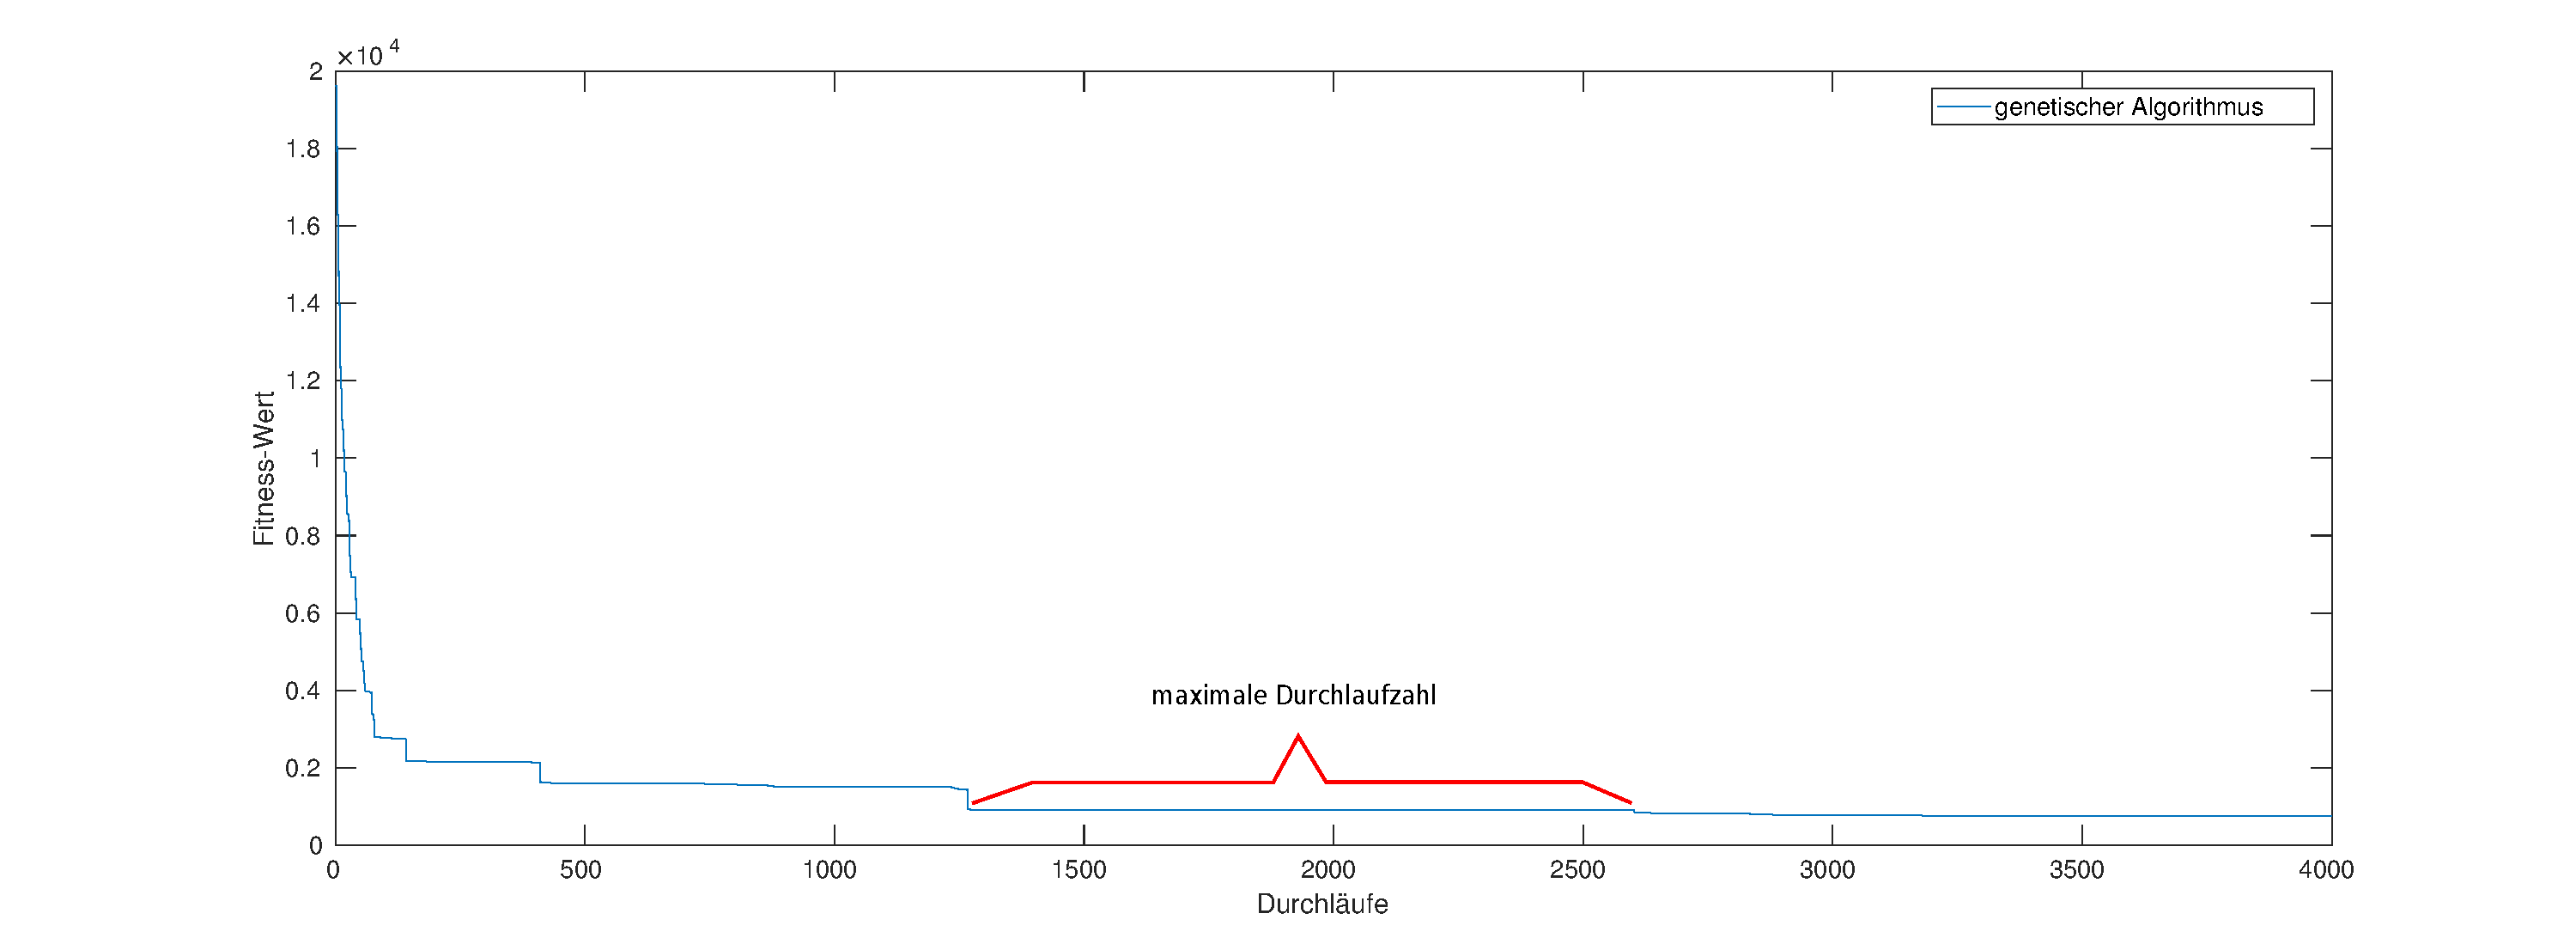
\includegraphics[width=\textwidth]{fig/iteration_analyse.pdf}
			\caption{Ermittlung der maximalen Durchlaufszahl}
			\label{fig:iteration_analyse}
		\end{figure}
	
	\item Größe der Population $N$\\
		Die Populationsgröße $N = 40$ wurde aus der Literatur \cite{grefenstette1986optimization} und Erfahrungswerte aus dem genetischen Instruktion-Scheduling entnommen.  
	
	\item Mutations-Wahrscheinlichkeit $w_M$\\
		Die Mutation ist dem Crossover untergeordnet und hebt die Flexibilität des Algorithmus. Dabei sind sehr kleine Werte zu wählen. Die Wahl fiel hierbei auf eine Wahrscheinlichkeit $w_M$ von einem Prozent. Dies bedeutet das $w_M * N * n$ Gene pro Population mutiert werden. Hierbei ist $n$ die Anzahl der Gene in einem Chromosom. Ist $w_M$ zu hoch gewählt, handelt es sich um eine Zufallssuche.
		
	\item Startwerte\\
		Die Startwerte haben einen erheblichen Einfluss auf die Laufzeit und Konvergenz des genetischen Algorithmus. Da die Gene zufallsgesteuert sind, kann auf diesen Parameter nur bedingt Einfluss genommen werden. Durch das Vorschalten der Heuristik und damit der Berechnung einer gültigen Register-Allokation, kann der Algorithmus bereits an einem besseren Ausgangsposition starten.(siehe Kapitel \ref{sub:startpop})
	\item Fitnessfunktion\\
		Den größten Einfluss auf die Funktion des Algorithmus hat jedoch die Fitness-Funktion. Diese ist ausschlaggebend für die Anpassung an das gegebene Problem und den Endwert des Algorithmus. Wird die Fitness-Funktion falsch gewählt, ist das Ergebnis des genetischen Algorithmus nicht aussagekräftig. 
\end{itemize}
 
\subsection{Startpopulation}
\label{sub:startpop}
Die Startpopulation besteht im Normalfall wie in Kapitel \ref{chap:aufbau} aus zufällig gewählten Genen. Hierbei werden nur Register verwendet, die nicht bereits von physikalischen Registern blockiert sind.
Um eine schnellere Konvergenz zu einem globalen Minimum zu gewährleisteten, wird ein Chromosom der Startpopulation durch ein Heuristik-Algorithmus bestimmt. Dadurch wird bereits bei einem lokalen Minimum gestartet und der genetische Algorithmus muss dieses nicht selbst finden. Ein Vergleich des Verlaufs der Fitness über der Anzahl der Durchläufe, kann in Abbildung \ref{fig:startpop} nachvollzogen werden und zeigt hierbei eine deutliche Zeitersparnis.

\begin{figure}[H]
	\centering
	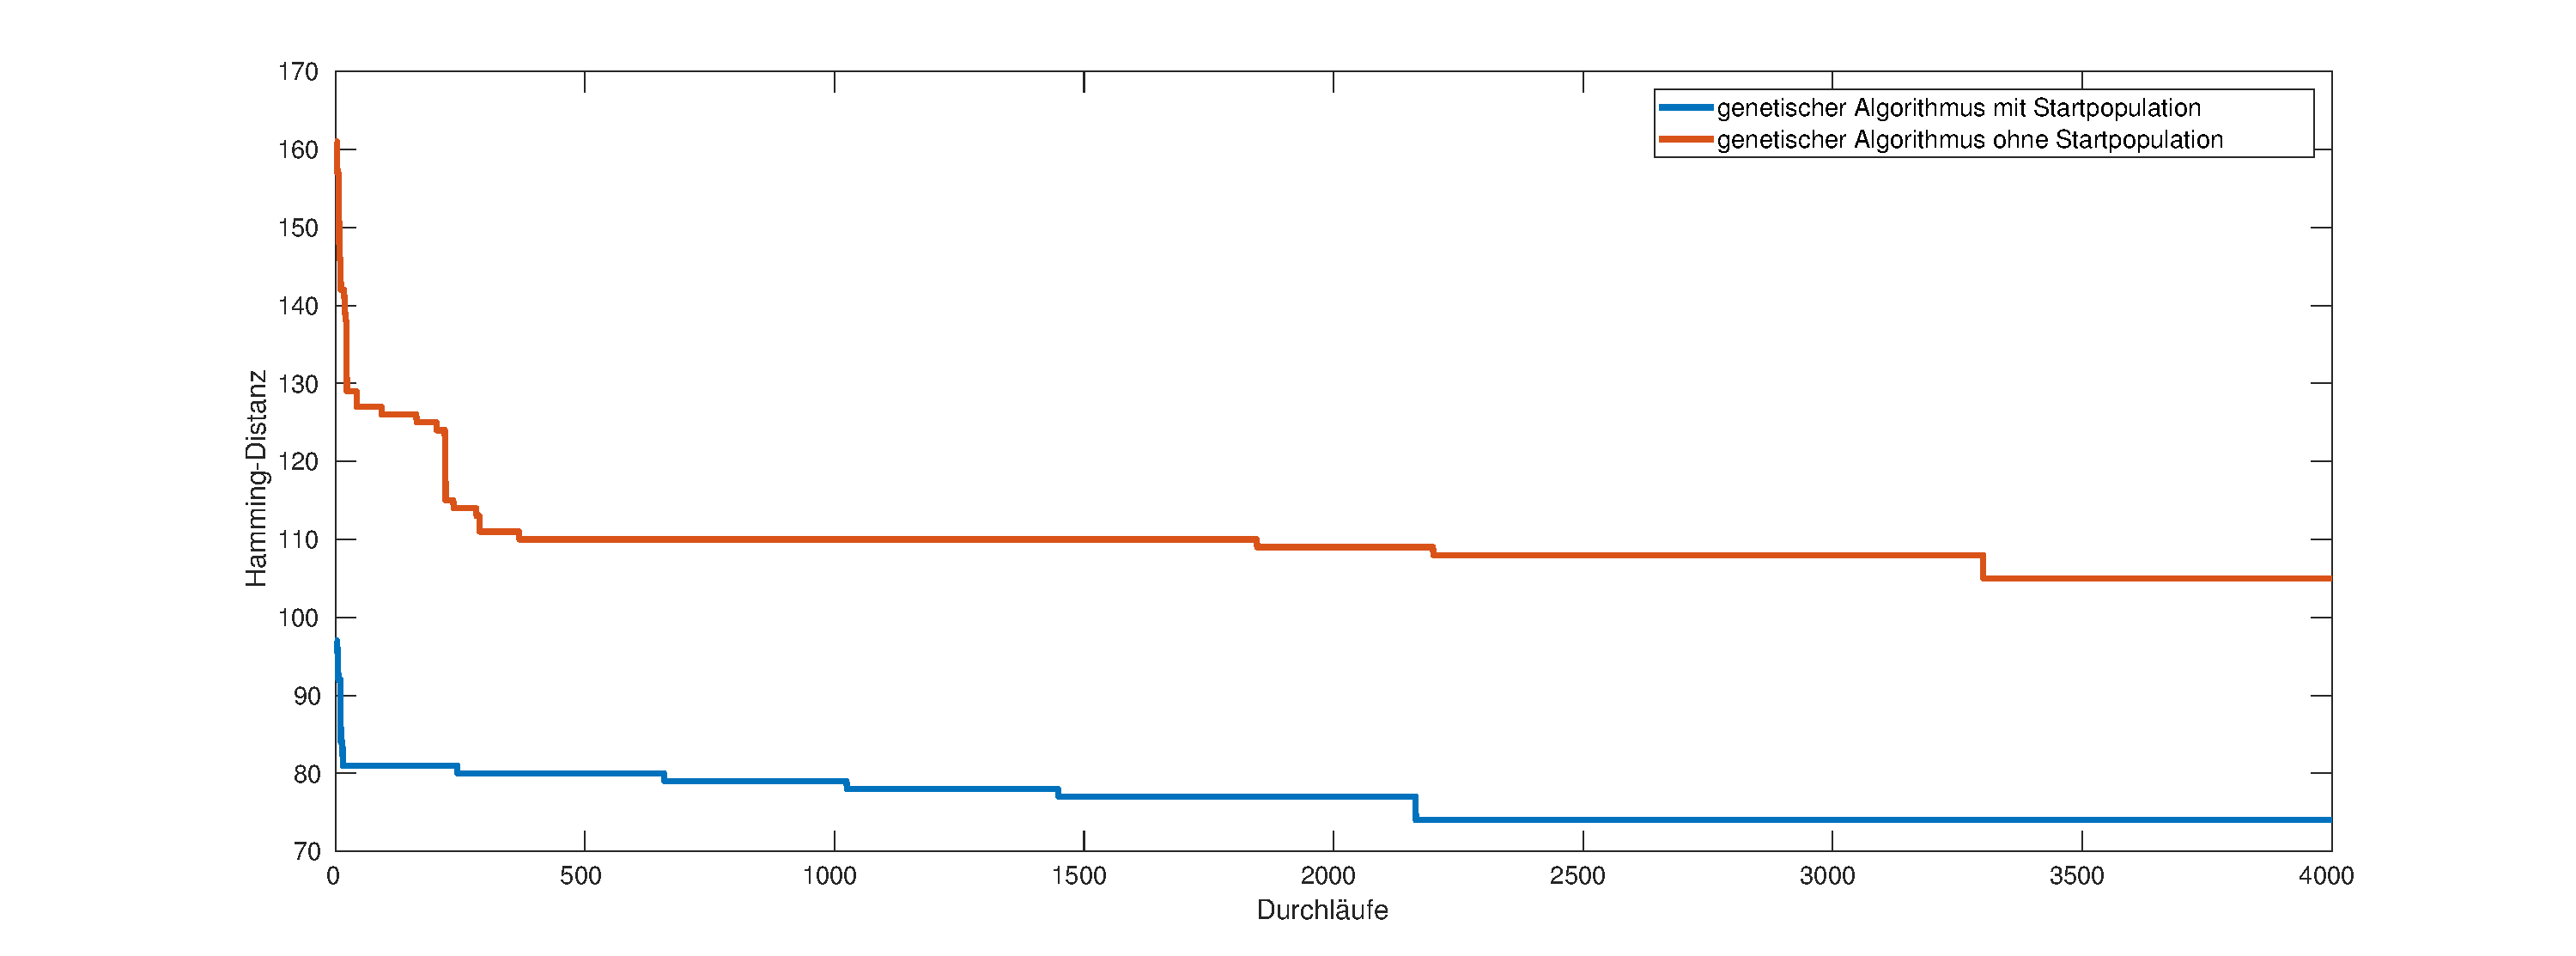
\includegraphics[width=\textwidth]{fig/startpop.pdf}
	\caption{Verlauf der Fitness mit und ohne Startpopulation}
	\label{fig:startpop}
\end{figure}

Nachteilig ist hierbei jedoch das durch ungeeignete Parameter der Algorithmus bei dem bereits sehr starken lokalen Minimum stagniert und keine Verbesserung mehr finden kann. Aus diesem Grund sollte beim Start mit der Heuristik eine höhere Mutations-Wahrscheinlichkeit eingesetzt werden um dieses Minimum dennoch zu überwinden.

\subsection{dynamische Anpassung}
Um eine schnellere Konvergenz gegen ein globales Minimum zu erreichen, wurde eine dynamische Anpassung der Parameter implementiert. Dies ist sinnvoll, da zu beginn die Suche auf einen großen Bereich ausgelegt werden muss, jedoch im weiteren Verlauf diese Parameter eventuell nicht mehr die schnellste Option darstellen. Aus diesem Grund wurde die Mutationsrate während der Berechnung angepasst. Zu beginn des Algorithmus werden viele bessere Lösungen als die der Startpopulation gefunden. Aus diesem Grund wird mit einer sehr kleinen Mutationsrate gestartet. Sobald für eine gewisse Anzahl an Durchläufen keine Verbesserung gefunden wurde, sprich der Algorithmus gegen ein lokales Minimum tendiert, wird die Mutations-Wahrscheinlichkeit erhöht. Dies hat zur Folge, dass die Suche nach geeigneten Genen breiter wird bzw. mehr Gene mutiert werden. Dadurch steigt die Wahrscheinlichkeit ein lokales Minimum zu überwinden an. Wird eine Verbesserung gefunden, wird die Mutationsrate auf den Startwert zurückgesetzt. Anderenfalls wird die Wahrscheinlichkeit weiter minimiert. Damit wird aus einer gezielten Suche wie in Abschnitt \ref{cap:parameter} erläutert eine Zufallssuche.
Das untenstehende Schaubild \ref{fig:dyn_genetic} zeigt die Optimierung, die durch diese Verfahren erreicht wurde. Hierbei wurden beide genetische Algorithmen mit dem selben Seed/Startwert ausgeführt, um die Versionen vergleichen zu können.

\begin{figure}[H]
	\centering
	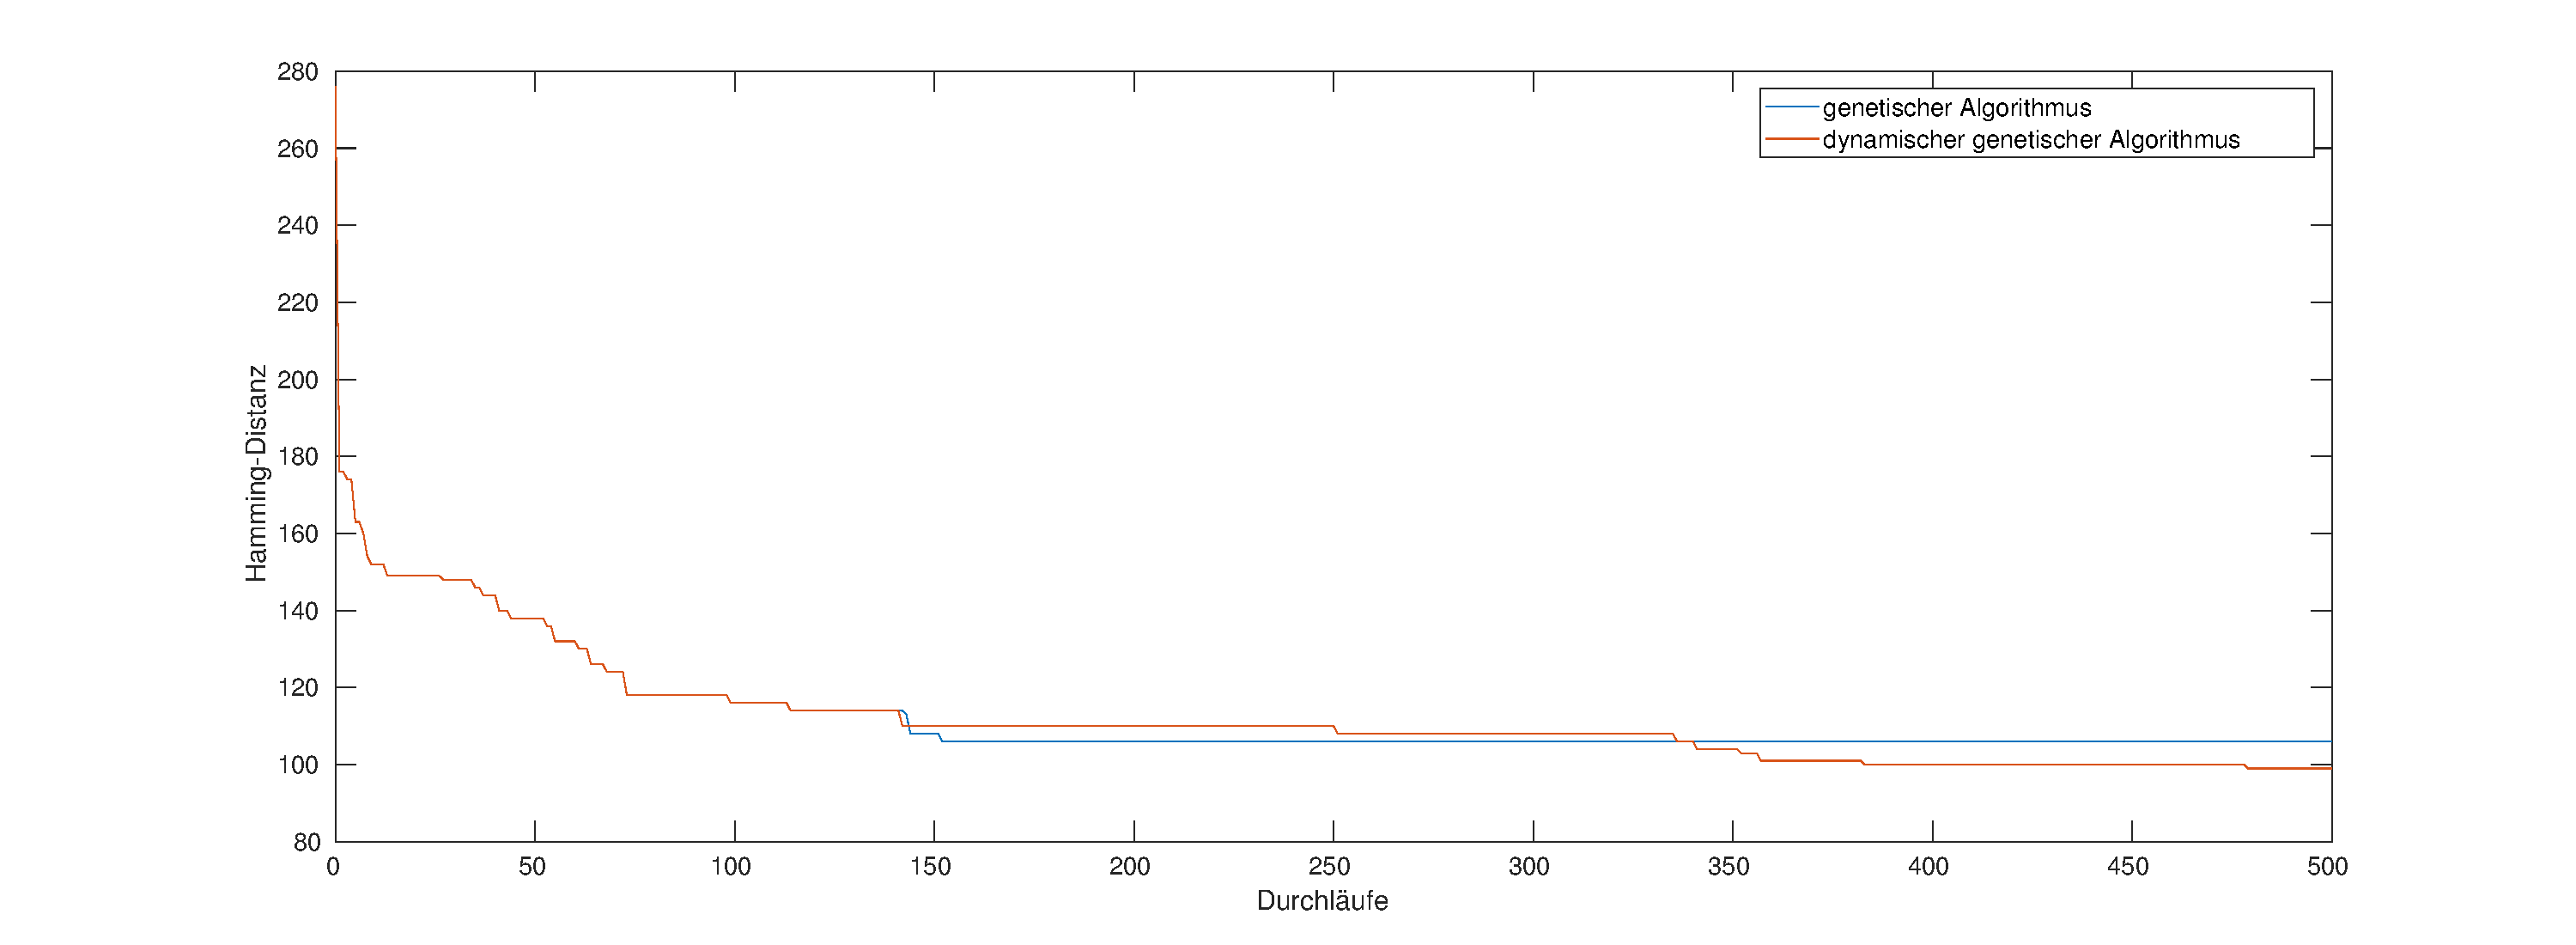
\includegraphics[width=\textwidth]{fig/dyn_genetic.pdf}
	\caption{dynamische Anpassung der Mutationsrate}
	\label{fig:dyn_genetic}
\end{figure}
 
\newpage
\subsection{Algorithmus Modi}
\begin{itemize}
	 \setlength{\itemsep}{-6pt}
	\item-E -> Register Allokations-Modus Heuristik
			\begin{itemize}
				\setlength{\itemsep}{-4pt}
				\item Alt
				\item Neu
			\end{itemize}
	\item-M -> Register Allokations-Modus Genetischer Algorithmus
		\begin{itemize}
			\setlength{\itemsep}{-4pt}
			\item Hamming-Distanz
			\item Load
			\item Hamming*Load
		\end{itemize}
	\item-G -> Auswahl der Algorithmen
			\begin{itemize}
				\setlength{\itemsep}{-4pt}
				\item Genetischer Algorithmus
				\item Heuristik
			\end{itemize}
	\item-D -> dynamischer Genetischer Algorithmus
	\item-H -> Heuristik als Startgen
	\item-U -> Mutation-Modus
				\begin{itemize}
					\setlength{\itemsep}{-4pt}
					\item Mutation auf Crossover-Gen
					\item Mutation auf Zufalls-Gen
				\end{itemize}
	\item-o -> Optimierungsgrad
			\begin{itemize}
				\setlength{\itemsep}{-4pt}
				\item o1 List Scheduling
				\item o2 Genetisches Scheduling 20 Gene
				\item o3 Genetisches Scheduling 100 Gene
				\item o4 Genetisches Scheduling 200 Gene
			\end{itemize}
	
\end{itemize}


	%Tabelle mit allen Modis 
	\begin{table}[htp]
		\centering
		\begin{tabular}{ccccccccc}
			\multicolumn{2}{l}{}                 & \multicolumn{7}{|l}{Modi}                                                               \\ 
			\multicolumn{2}{c}{Algorithmus-Konfig.}  & \multicolumn{1}{|c}{-E} & \multicolumn{1}{c}{-M} & \multicolumn{1}{c}{-G} & \multicolumn{1}{c}{-D} & \multicolumn{1}{c}{-H} & \multicolumn{1}{c}{-U} & \multicolumn{1}{c}{-o} \\ 
			\hline
		\multicolumn{2}{l}{Heuristik alt}  & \multicolumn{1}{|c}{0} & \multicolumn{1}{c}{1} & \multicolumn{1}{c}{0} & \multicolumn{1}{c}{X} & \multicolumn{1}{c}{X} & \multicolumn{1}{c}{X} & \multicolumn{1}{c}{1} \\
		\multicolumn{2}{l}{Heuristik neu}  & \multicolumn{1}{|c}{1} & \multicolumn{1}{c}{1} & \multicolumn{1}{c}{0} & \multicolumn{1}{c}{X} & \multicolumn{1}{c}{X} & \multicolumn{1}{c}{X} & \multicolumn{1}{c}{1} \\ 
		\multicolumn{2}{l}{Genetischer Algo. Hamming-Fitness}  & \multicolumn{1}{|c}{1} & \multicolumn{1}{c}{1} & \multicolumn{1}{c}{1} & \multicolumn{1}{c}{0} & \multicolumn{1}{c}{0} & \multicolumn{1}{c}{0} & \multicolumn{1}{c}{2-4} \\
			\multicolumn{2}{r}{Heuristik als Startpop.}  & \multicolumn{1}{|c}{1} & \multicolumn{1}{c}{1} & \multicolumn{1}{c}{1} & \multicolumn{1}{c}{0} & \multicolumn{1}{c}{1} & \multicolumn{1}{c}{0} & \multicolumn{1}{c}{2-4} \\
			\multicolumn{2}{r}{dynamischer Genetischer Algo.}  & \multicolumn{1}{|c}{1} & \multicolumn{1}{c}{1} & \multicolumn{1}{c}{1} & \multicolumn{1}{c}{1} & \multicolumn{1}{c}{0} & \multicolumn{1}{c}{0} & \multicolumn{1}{c}{2-4} \\
		\multicolumn{2}{l}{Genetischer Algo. Load-Fitness}  & \multicolumn{1}{|c}{1} & \multicolumn{1}{c}{2} & \multicolumn{1}{c}{1} & \multicolumn{1}{c}{0} & \multicolumn{1}{c}{0} & \multicolumn{1}{c}{0} & \multicolumn{1}{c}{2-4} \\ 
		\multicolumn{2}{l}{Genetischer Algo. Hamming*Load-Fitness}  & \multicolumn{1}{|c}{1} & \multicolumn{1}{c}{3} & \multicolumn{1}{c}{1} & \multicolumn{1}{c}{0} & \multicolumn{1}{c}{0} & \multicolumn{1}{c}{0} & \multicolumn{1}{c}{2-4}                     
		\end{tabular}
		\newline
		\caption{Algorithmus-Konfiguration}
		\label{tab:algo_conifg}
	\end{table}

